\section{Durchführung}

\subsection{Angaben zur Apparatur}

\begin{figure}[H]
    \centering
    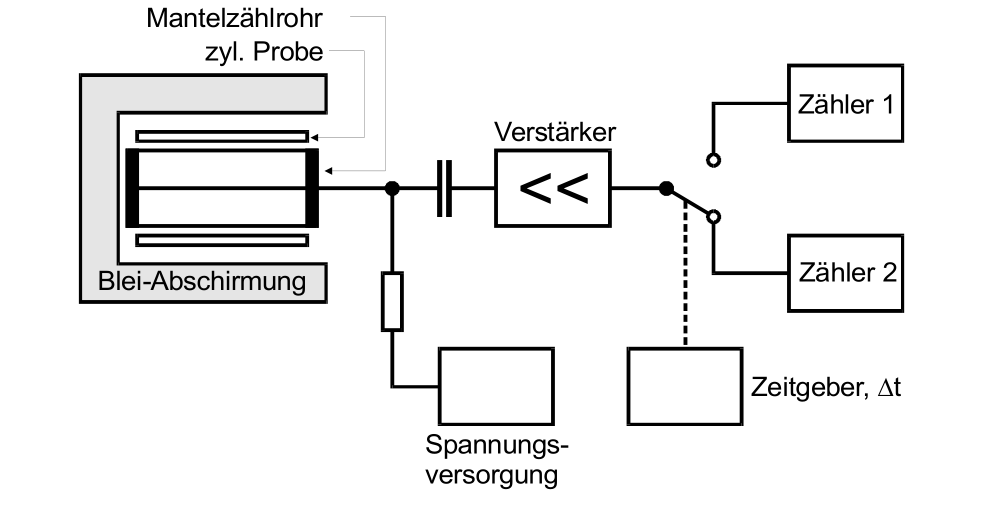
\includegraphics[width=0.75\textwidth]{images/Theorie3.PNG}
    \caption{Schematische Darstellung des Versuchsaufbaus \protect \cite{V702}.}
    \label{img:Apparatur}
\end{figure}

\noindent Die Messungen werden mit der Apperatur aus Abbildung(\ref{img:Apparatur}) durchgeführt. Mittels eines Geiger-Müller-Zählrohrs wird ein konstanter 
Teil der durch die Proben ausgestrahlten $\beta$- und $\gamma$-Strahlung detektiert. Das Zählrohr ist mit Blei abgeschirmt um den Nullefekt zu verringern.
Die einzelnen Impulse des Zählrohrs werden verstärkt und dann abwechselnd an den Zählern 1 und 2 gezählt. Das Wechseln zwischen Zähler 1 und 2 
geschieht durch den Zeitgeber. Dort wird das Zeitintervall $\Delta t$ definiert.
\subsection{Nullefekt}
\noindent Durch Höhenstrahlung und natürliche Radioaktivität misst das Zählrohr auch einkommende Strahlung selbst wenn keine aktivierte Probe in der 
Nähe des Zählrohrs ist. Diese Impulse stören bei der Berechnung der Halbwertszeiten. Um diesen Nullefekt zu umgehen muss er genau bestimt werden, 
dazu wird mit einem Messintervall von t=300s, 7 mal die Hintergrundstrahlung gemessen.


\subsection{Vanadium}

\noindent Zur Bestimmung einer Halbwertszeit eines Isotops mit einfachen Zerfall wird in diesem Versuch Vanadium genutzt. Dazu wird die Probe aktiviert,
in das Geiger-Müller-Zählrohr gesteckt und dann in $\Delta t$ = 30s Messintervallen die Strahlungsteilchen gemessen. Dies wird solange gemacht 
bis sich die Strahlung nicht mehr von der Hintergrundstrahlung unterschieden lässt.

\subsection{Rhodium}

\noindent Zur Bestimmung der Halbwertszeiten eines Isotopengemischs wird Rhodium genutzt. Die Messung wird analog zum Vanadium durchgeführt, 
nur die Messintervalle werden auf $\Delta t$=15s halbiert.